\chapter{Graphical User Interface}


\section{Motivation}
A \gls{gui} framework has been developed during the master thesis.
There were two main motivations behind this.

In order to operate a camera system in real time it is pretty usefull to be able to see what the camera sees.
During the \preproject a simple way of interacting with the system from a phone over \gls{ssh} through an app called juiceSSH was tested \cite[32]{martensPortableSensorRig2022}.
This app was tested more in the beginning of the master thesis, and several usefull snippets were saved in the app.
Although the text interface was sufficient to start and stop the recording and verify that images were saved, the lack of a graphical interface made it difficult to verify that the camera was recording what it was supposed to.
Thus a \gls{gui} is needed.

In a more general context a need for an efficient way to interact with programs and visualize data on remote computers was identified.
The \jx has been the current platform for the master thesis, but during future work other remote computers will be used.
A powerful workstation with a \todo was aquired last fall to be used for training and inference of \gls{ai} models during future Ph.D.
work.
The workstation is headless, that is it has no monitor, keyboard or mouse, as we are a couple of people that will be using it.

\subsection{Specifications}
There are a lot of different options to choose from when it comes to \gls{gui} frameworks.
But the following requirements were identified:
\begin{itemize}
    \item Access from all devices including smartphone
    \item Easy to develop
    \item Capable of real time visualization
    \item Reasonably efficient
    \item Easily customizable
\end{itemize}
From the forst requirement it was clear that the solution would be web based as this it is the easiest way to make a \gls{gui} that is accessible from different types of devices.
Using a \gls{js} framework like React, Vue or Svelte would probably have been a good choice, but with very little personal experience using \gls{js} it appeared too ambitious to learn a new framework in a new language.
\dash was chosen as it is based on \py, making the learning curve less steep.


\dash is not designed for real time applications and lacks native support for \glsps{websocket}.
Fortunately a group of people have developed a package called \texttt{dash-extensions} that adds support for \glsps{websocket} to \dash \cite{eriksenDashExtensions}.
To improve performance the thread baced backend of \dash, Flask, was replaced with asynchronous \gls{quart}.

\subsection{Replacing Flask backend with Quart}
The first step in the development of the \guif was to replace the Flask backend with \gls{quart}.
As the comperaison in Listing \ref{listing:concurrency_test} shows, \gls{asyncio} baseded code has significantly less overhead than asynchronous code based threads in \py.


Snehil Vijay has created a fork of \dash, called \gls{async-dash}, that replaces the Flask backend with \gls{quart} \cite{vijaySnehilvjAsyncdash2023}.
As \gls{quart} is created to be a drop in replacement for Flask, this fork
Another project aimed at making \gls{dash} run \gls{quart} called \code{dash_deviced} was also tested, but was not as easy to use as the fork by Snehil Vijay, and did not have any acivity for the last  \cite{legrandCodeFrequencyRichlegrand}.

\subsection{Adding support for websockets}
WebSockets is technology that enables two-way communication between a user's browser and a server.
\cite{farhutsWebSocketsBeginnersPart2019}.
Unlike traditional HTTP, which requires the browser to constantly request information from the server, WebSockets allow for a persistent connection as visualized in Figure \ref{fig:websockets_vs_http}\cite{farhutsWebSocketsBeginnersPart2019}.
This means that the server can send updates to the browser in real-time without the need for continuous requests.
\begin{figure}[H]
    \centering
    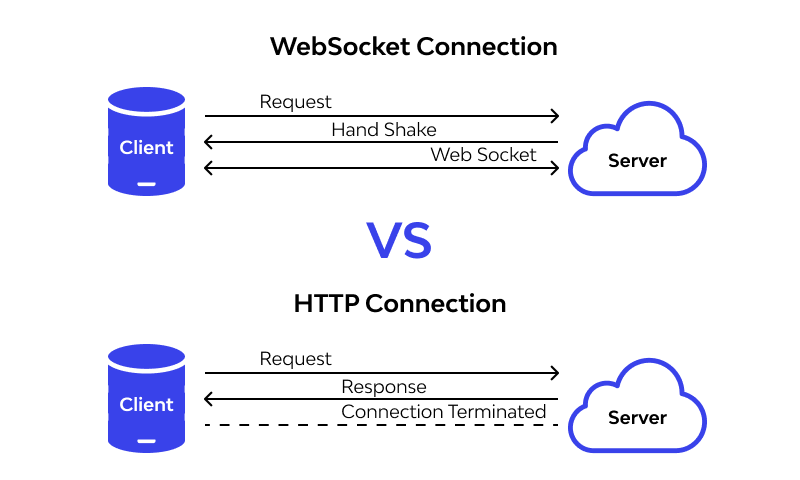
\includegraphics[width=0.6\textwidth]{figures/gui/http_vs_ws.png}
    \caption{WebSockets Vs HTTP \cite{wallarmWebSocketVsHTTP}}
    \label{fig:websockets_vs_http}
\end{figure}

One of the main motivations for using \gls{quart} as backend is that it supports \glspl{ws} nativly \cite{quartUsingWebsocketsQuart}.
However, \dash does not support \gls{ws} out of the box, so this feature had to be added by integrating the \gls{dashextensions} into the project, that enables \gls{ws} support \cite{eriksenDashExtensionsWebSocket}

\subsection{Websockets through Quart and Dash-Extentions}
\cite{plotlyLiveUpdatesDash}








\subsection{Multi-page apps}
Dash supports multi-page apps, making it possible to create a web application with multiple pages that the user can navigate between \cite{plotlyMultiPageAppsURL}.
The primary intended use for this was to have separate pages on the \srgui.
One for cameara control and visualization, one for starting and monitoring recordings and one for general monitoring of the system.
A developer named Ann Marie Ward has created a set of examples on how to work with multi-page apps that was used as a starting point \cite{wardExamplesMultipageApps03Jul22}.

One major issue was that \gls{async-dash} did not work with multi-page apps.
Fortunately there is an open pull-request that fixes this issue \cite{lekAddFlaskRequest2022}.

